% H2 Projection method — Persian solution, XeLaTeX + xepersian
\documentclass[12pt,a4paper]{article}
\usepackage{amsmath,amssymb}
\usepackage{booktabs}
\usepackage{graphicx}
\usepackage{geometry}
\geometry{margin=25mm}
\usepackage[hidelinks]{hyperref}
\usepackage{xepersian}
\settextfont{Vazirmatn}
\setdigitfont{Vazirmatn}
\usepackage{setspace}
\setstretch{1.25}
\begin{document}

\begin{center}
{\Large\bfseries روش پروجکشن (گام کسری) چورین ۱۹۶۷\par}
\vspace{1ex}
{\large توضیح با نگارش دکتر، اثبات معادلهٔ پواسون و اعتبارسنجی عددی\par}
\vspace{1ex}
{\small امیر مرادی\\
درس مدل‌سازی توربولانس · گروه مهندسی مکانیک\\
استاد: دکتر ثبت‌قدم · پاییز ۱۴۰۵\\
۶ آبان ۱۴۰۵ / \lr{2026-10-28}\par}
\end{center}

\begin{center}{\large\bfseries چکیده}\end{center}
مسئله این است: در جریان تراکم‌ناپذیر، فشار معادلهٔ تکامل زمانی ندارد و فقط
«نگهبان» شرط بی‌واگرایی است. روش پروجکشن این مشکل را با دو نیم‌گام حل می‌کند:
اول سرعت را بدون جملهٔ فشار جلو می‌بریم و یک «سرعت میانی» می‌سازیم که
معمولاً واگرا دارد؛ بعد با حل یک معادلهٔ پواسون برای یک فشار کمکی، فقط یک
میدان گرادیانی به آن اضافه می‌کنیم تا واگرایی دقیقاً صفر شود. این مقاله
هر سه گام را با همان نمادهای جزوهٔ دکتر می‌نویسد، معادلهٔ پواسون را از
گرفتن واگرایی از گام تصحیح «اثبات» می‌کند، یک دام علامت رایج در رونوشت
جزوه را صریحاً اصلاح می‌کند، و با کد پایتون نشان می‌دهد که پس از تصحیح،
بیشینهٔ واگرایی در حد \lr{$10^{-14}$} و خطای انرژی تیلور--گرین در حد
\lr{$2\times10^{-4}$} است.

\noindent\textbf{واژگان کلیدی:} روش پروجکشن؛ گام کسری؛ چورین؛ معادلهٔ پواسون؛
فشار کاذب؛ جریان تراکم‌ناپذیر؛ سرعت میانی.

\section{جواب اول}
روش پروجکشن یعنی: \textbf{فشار را از گام سرعت جدا کن، سرعت میانی بساز،
بعد با پواسون آن را روی فضای بی‌واگرا «تصویر» کن.} سه فرمول، با نگارش دکتر،
چنین‌اند (چگالی \lr{$\rho=1$} گرفته شده است):
\begin{align}
\frac{\hat{\mathbf{u}}^{n+1}-\mathbf{u}^n}{\Delta t}
&= -(\mathbf{u}^n\cdot\nabla)\mathbf{u}^n
   + \nu\nabla^2\mathbf{u}^n
   &&\text{(۱) سرعت میانی} \label{eq:predictor}\\
\nabla^2\pi &= -\frac{\nabla\cdot\hat{\mathbf{u}}^{n+1}}{\Delta t}
   &&\text{(۲) پواسون برای فشار کاذب} \label{eq:poisson}\\
\mathbf{u}^{n+1} &= \hat{\mathbf{u}}^{n+1} + \Delta t\,\nabla\pi
   &&\text{(۳) تصحیح} \label{eq:corrector}
\end{align}
در اینجا \lr{$\hat{\mathbf{u}}^{n+1}$} سرعت میانی، \lr{$\pi$} فشار کاذب
\lr{(pseudo-pressure)} و \lr{$\Delta t$} گام زمانی است. نتیجهٔ اصلی که باید
ثابت شود این است: اگر \lr{$\pi$} از \eqref{eq:poisson} به دست آید، آنگاه
از \eqref{eq:corrector} حتماً \lr{$\nabla\cdot\mathbf{u}^{n+1}=0$} می‌شود.
اثباتش فقط دو خط است و در بخش ۴ آمده است.

\section{صورت مسئله و نقطهٔ شروع: اویلر پیشرو}
معادلات ناویر--استوکس تراکم‌ناپذیر (بدون در نظر گرفتن نیروی حجمی، یا با
جذب آن در سمت راست) چنین‌اند:
\begin{equation}
\frac{\partial\mathbf{u}}{\partial t}
= -(\mathbf{u}\cdot\nabla)\mathbf{u} - \nabla p + \nu\nabla^2\mathbf{u},
\qquad
\nabla\cdot\mathbf{u}=0.
\label{eq:ns}
\end{equation}
نکتهٔ کلیدی: معادلهٔ دوم مشتق زمانی ندارد. پس فشار \lr{$p$} مثل سرعت
«جلو برده» نمی‌شود؛ فشار در هر لحظه باید چنان انتخاب شود که شرط
\lr{$\nabla\cdot\mathbf{u}=0$} برقرار بماند. به همین دلیل فشار را
«ضرب‌کنندهٔ لاگرانژِ» شرط تراکم‌ناپذیری می‌نامند: خودش متغیر حالت نیست،
ابزارِ تحمیلِ قید است.

جزوه از همین‌جا شروع می‌کند. برای یک مؤلفهٔ سرعت، با اویلر پیشرو
\lr{(forward Euler)} داریم:
\begin{equation}
\left.\frac{\partial u_j}{\partial t}\right|_{t_0} = (\mathrm{RHS})_{t_0}
\quad\Longrightarrow\quad
\frac{u_j^1-u_j^0}{\Delta t} \approx (\mathrm{RHS})_{t_0}
\quad\Longrightarrow\quad
\boxed{\,u_j^1 = u_j^0 + \Delta t\,(\mathrm{RHS})_{t_0}\,}.
\label{eq:euler}
\end{equation}
یعنی مقدار جدید برابر مقدار قدیم به‌علاوهٔ «نرخ تغییر در لحظهٔ قدیم، ضرب‌در
گام زمانی». روش پروجکشن همین ایده را به‌کار می‌برد، با این تفاوت که جملهٔ
فشار را در نیم‌گام اول کنار می‌گذارد و در نیم‌گام دوم، جداگانه، وارد می‌کند.
به همین دلیل به آن «گام کسری» \lr{(fractional step)} هم می‌گویند: یک گام
کامل زمانی، به دو گام کسری شکسته شده است.

\begin{table}[htbp]
\centering
\caption{نمادها، دقیقاً با نگارش جزوه}
\begin{tabular}{cl}
\toprule
نماد & معنی \\
\midrule
\lr{$\mathbf{u}^n$} & سرعت فیزیکی در گام \lr{$n$}، بی‌واگرا: \lr{$\nabla\cdot\mathbf{u}^n=0$} \\
\lr{$\hat{\mathbf{u}}^{n+1}$} & سرعت میانی \lr{(intermediate velocity)}؛ هنوز فیزیکی نیست \\
\lr{$\pi$} & فشار کاذب \lr{(pseudo-pressure)}؛ گرادیانش سرعت را اصلاح می‌کند \\
\lr{$\nu$} & لزجت سینماتیکی \\
\lr{$\Delta t$} & گام زمانی \\
\bottomrule
\end{tabular}
\end{table}

\section{گام ۱: سرعت میانی؛ چرا واگرا دارد؟}
در گام ۱، معادلهٔ مومنتم را بدون جملهٔ فشار جلو می‌بریم:
\begin{equation}
\hat{\mathbf{u}}^{n+1}
= \mathbf{u}^n + \Delta t\left[
-(\mathbf{u}^n\cdot\nabla)\mathbf{u}^n + \nu\nabla^2\mathbf{u}^n
\right].
\end{equation}
جملهٔ اول سمت راست، جابه‌جایی (همرفت) است؛ جملهٔ دوم، پخش لزجتی است.
چون جملهٔ \lr{$-\nabla p$} حذف شده، هیچ مکانیزمی در این گام واگرایی را
کنترل نمی‌کند. پس در حالت کلی
\begin{equation}
\nabla\cdot\hat{\mathbf{u}}^{n+1} \neq 0,
\end{equation}
و \lr{$\hat{\mathbf{u}}$} سرعتِ یک جریان تراکم‌ناپذیرِ واقعی نیست؛ فقط یک
«حدس میانی» است که اثر همرفت و لزجت را در خود دارد. اشتباه رایج این است
که \lr{$\hat{\mathbf{u}}$} را همان جواب گام بعد بدانیم؛ نیست. کارِ فشار،
دقیقاً پاک‌کردن همین واگراییِ اضافه است.

\section{گام ۲ و ۳: اثبات معادلهٔ پواسون و صفر شدن واگرایی}
حالا گام تصحیح دکتر را می‌نویسیم و از آن، معادلهٔ پواسون را «استخراج»
می‌کنیم، نه اینکه آن را از پیش فرض بگیریم. گام تصحیح:
\begin{equation}
\mathbf{u}^{n+1} = \hat{\mathbf{u}}^{n+1} + \Delta t\,\nabla\pi.
\label{eq:corr2}
\end{equation}
از دو طرف واگرایی می‌گیریم. واگرایی و مشتق زمانی/مکانی خطی‌اند و
\lr{$\nabla\cdot(\nabla\pi)=\nabla^2\pi$} است، پس:
\begin{equation}
\nabla\cdot\mathbf{u}^{n+1}
= \nabla\cdot\hat{\mathbf{u}}^{n+1} + \Delta t\,\nabla^2\pi.
\label{eq:divcorr}
\end{equation}
حالا شرط فیزیکی را تحمیل می‌کنیم: سرعتِ نهایی باید بی‌واگرا باشد،
\lr{$\nabla\cdot\mathbf{u}^{n+1}=0$}. جای‌گذاری در \eqref{eq:divcorr}:
\begin{equation}
0 = \nabla\cdot\hat{\mathbf{u}}^{n+1} + \Delta t\,\nabla^2\pi
\quad\Longrightarrow\quad
\boxed{\,\nabla^2\pi = -\frac{\nabla\cdot\hat{\mathbf{u}}^{n+1}}{\Delta t}\,}.
\end{equation}
همین است: معادلهٔ پواسون. سمت راستش معلوم است (واگرایی سرعت میانی،
تقسیم بر گام زمانی) و مجهولش \lr{$\pi$} است. وقتی این معادله را در کل
دامنه حل کردیم، \lr{$\pi$} را داریم؛ با \eqref{eq:corr2} سرعت را اصلاح
می‌کنیم؛ و برای اطمینان، واگرایی نهایی را دوباره حساب می‌کنیم:
\begin{equation}
\nabla\cdot\mathbf{u}^{n+1}
= \nabla\cdot\hat{\mathbf{u}}^{n+1}
+ \Delta t\left(-\frac{\nabla\cdot\hat{\mathbf{u}}^{n+1}}{\Delta t}\right)
= 0.
\qquad\blacksquare
\end{equation}
این، اثبات کاملِ ادعاست. تفسیر هندسی‌اش هم ساده است: تصحیح
\lr{$\Delta t\,\nabla\pi$} یک میدان «خالصِ گرادیانی» است. هر میدان برداری
را می‌توان به یک بخش بی‌واگرا و یک بخش گرادیانی تجزیه کرد (تجزیهٔ هلمهولتز)؛
پواسون دقیقاً همان بخش گرادیانیِ \lr{$\hat{\mathbf{u}}$} را پیدا و کم
می‌کند. به همین دلیل به کل روش «پروجکشن» می‌گویند: \lr{$\hat{\mathbf{u}}$}
را بر فضای میدان‌های بی‌واگرا تصویر می‌کنیم.

\subsection*{دام علامت؛ اصلاح صریح یک رونوشت}
در رونوشت دوم جزوه، گام تصحیح با علامت منفی نوشته شده است،
\lr{$\mathbf{u}^{n+1}=\hat{\mathbf{u}}^{n+1}-\Delta t\,\nabla\pi$}، ولی
پواسون همچنان با علامت منفی آمده است. آن دو با هم سازگار نیستند: با آن
ترکیب، از \eqref{eq:divcorr} با علامت منفی،
\lr{$\nabla\cdot\mathbf{u}^{n+1}=2\,\nabla\cdot\hat{\mathbf{u}}$} می‌شود،
نه صفر. فقط یکی از دو جفت زیر درست است:

\begin{table}[htbp]
\centering
\caption{دو جفت علامتِ سازگار؛ هرگز آن‌ها را با هم قاطی نکنید}
\begin{tabular}{ccc}
\toprule
قرارداد & تصحیح & پواسون \\
\midrule
الف) نگارش دکتر (این مقاله) &
\lr{$\mathbf{u}^{n+1}=\hat{\mathbf{u}}+\Delta t\nabla\pi$} &
\lr{$\nabla^2\pi=-\nabla\cdot\hat{\mathbf{u}}/\Delta t$} \\
ب) کتاب‌های استاندارد &
\lr{$\mathbf{u}^{n+1}=\hat{\mathbf{u}}-\Delta t\nabla p$} &
\lr{$\nabla^2 p=+\nabla\cdot\hat{\mathbf{u}}/\Delta t$} \\
\bottomrule
\end{tabular}
\end{table}

این دو، یک روش‌اند با تغییر نام: در قرارداد الف،
\lr{$\pi=-p^{n+1}$} (برای \lr{$\rho=1$}؛ در حالت کلی
\lr{$\pi=-p^{n+1}/\rho$}). پس \lr{$\pi$} «فشار کاذب» نامیده می‌شود:
خودش فشار فیزیکی نیست، بلکه منفیِ آن است، و فقط گرادیانش در روش به کار
می‌رود. کد این مقاله قرارداد الف را پیاده می‌کند و فشار فیزیکی را
\lr{$p=-\pi$} گزارش می‌کند.

\section{شرط مرزی پواسون و یکتایی \lr{$\pi$}}
\lr{$\pi$} فقط از راه گرادیانش وارد سرعت می‌شود؛ پس افزودن یک ثابت به
\lr{$\pi$} هیچ تغییری در سرعت نمی‌دهد. معادلهٔ پواسون هم برای
\lr{$\pi$} یکتا نیست، مگر یک قید اضافه بگذاریم، مثلاً میانگین
\lr{$\pi$} صفر باشد یا مقدارش در یک نقطه ثابت شود. در کد تناوبی، مُد
صفرِ فوریهٔ \lr{$\pi$} صفر گذاشته شده است.

شرط مرزی نوعِ نیومنِ \lr{$\pi$} از گام تصحیح به دست می‌آید. مؤلفهٔ عمودی
\eqref{eq:corr2} روی مرز:
\begin{equation}
\frac{\partial\pi}{\partial n}
= \frac{(\mathbf{u}^{n+1}-\hat{\mathbf{u}}^{n+1})\cdot\mathbf{n}}{\Delta t}.
\end{equation}
برای دیوارهٔ نفوذناپذیر، \lr{$\mathbf{u}^{n+1}\cdot\mathbf{n}=0$}، پس
\lr{$\partial\pi/\partial n=-\hat{\mathbf{u}}\cdot\mathbf{n}/\Delta t$}.
این یک شرط مرزی «مصنوعی» است: از فیزیک فشار نیامده، از نیازِ روش به
بی‌واگرا شدن آمده است. همچنین برای حل‌پذیری مسئلهٔ نیومن باید شرط
سازگاریِ قضیهٔ واگرایی برقرار باشد:
\lr{$\int_\Omega\nabla\cdot\hat{\mathbf{u}}\,dV
=\int_{\partial\Omega}\hat{\mathbf{u}}\cdot\mathbf{n}\,dS$}؛
در دامنهٔ تناوبی، میانگین سمت راست پواسون خودبه‌خود صفر است.

\section{روش حل عددی و بازتولید}
کد \lr{\texttt{notebooks/projection\_method.py}} روش را در دامنهٔ تناوبی
\lr{$[0,2\pi)\times[0,2\pi)$} با مشتق‌های طیفی \lr{(FFT)} پیاده می‌کند؛
یعنی پواسون در فضای فوریه، مُدبه‌مُد، با تقسیم بر \lr{$-k^2$} حل می‌شود.
دو آزمون از پیش ثبت‌شده در \lr{\texttt{protocols/H2\_frozen.md}} آمده است:

\textbf{آزمون الف — پروجکشن خالص:} میدان میانی را عمداً خراب می‌کنیم:
میدان دقیق تیلور--گرین به‌علاوهٔ گرادیان
\lr{$\phi=0.3\sin x\sin y$}. یک گام پواسون و تصحیح باید میدان دقیق را
برگرداند و واگرایی را به حد دقت ماشین برساند.

\textbf{آزمون ب — تیلور--گرین زمانی:} جریان دقیق
\lr{$\mathbf{u}=(\sin x\cos y,\,-\cos x\sin y)\,e^{-2\nu t}$}،
با \lr{$\nu=0.1$}، شبکهٔ \lr{$64\times64$}، \lr{$\Delta t=0.005$} تا
\lr{$t=1$}. جملهٔ غیرخطی این جریان، خالصِ گرادیانی است؛ پس دقیقاً همان
چیزی است که پروجکشن باید حذف کند. انرژی جنبشی دقیق
\lr{$E(t)=\frac14 e^{-4\nu t}$} است.

\section{نتایج}
\begin{figure}[htbp]
\centering
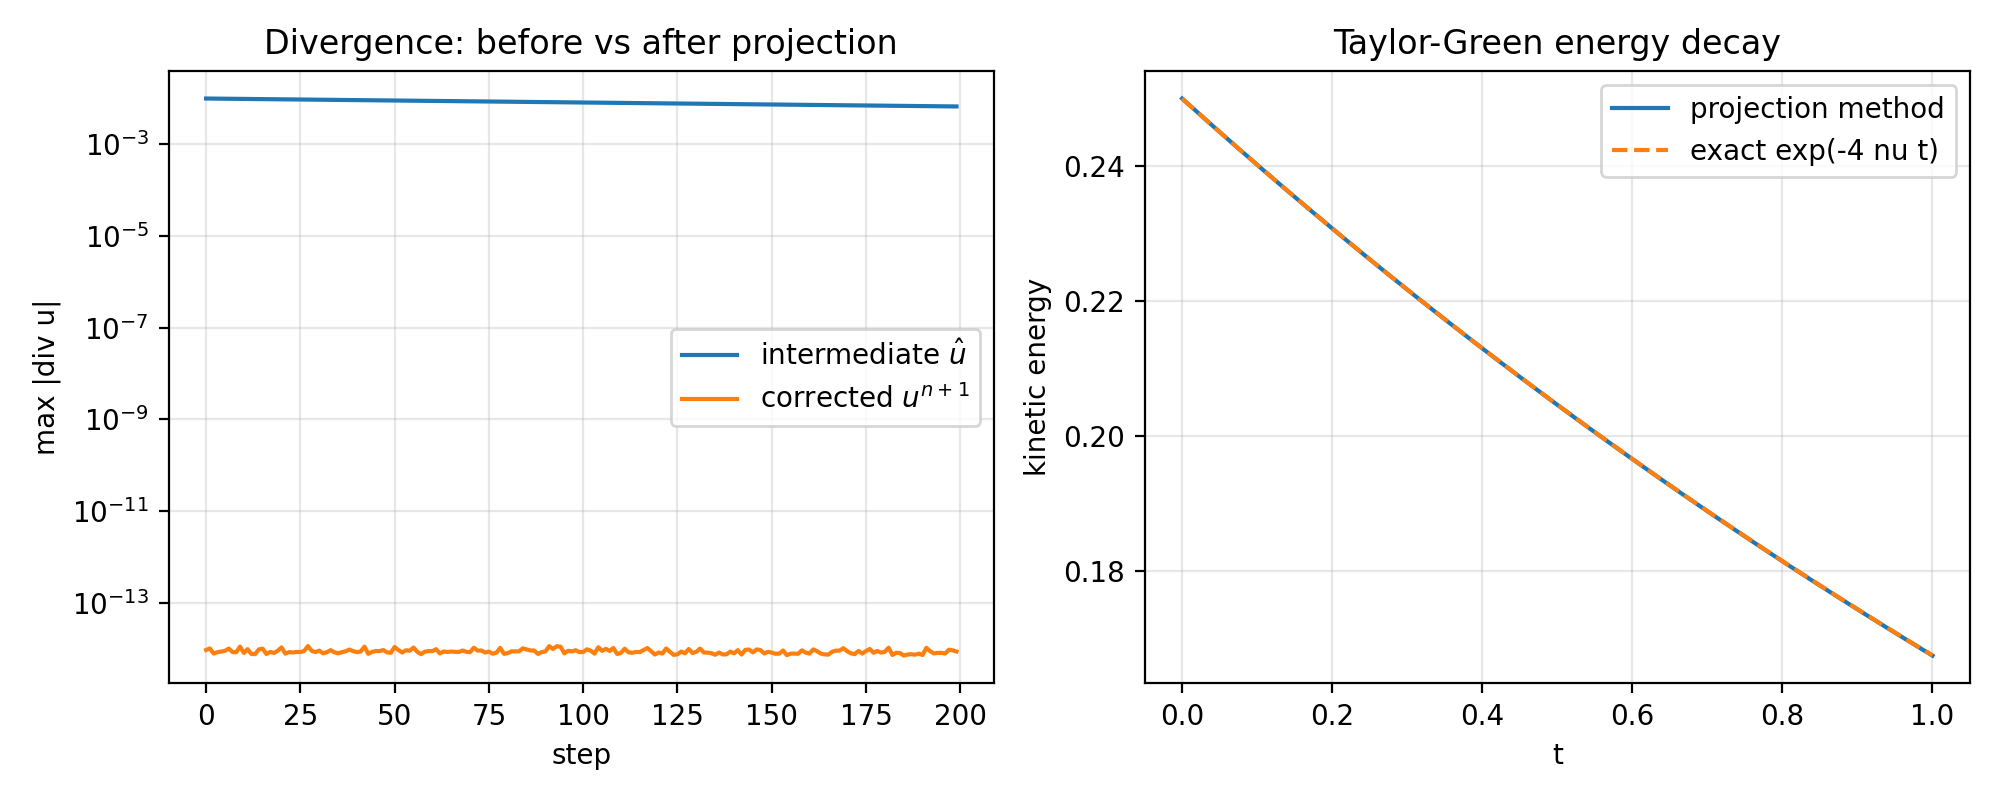
\includegraphics[width=.95\linewidth]{../results/figures/divergence_energy.png}
\caption{چپ: بیشینهٔ واگرایی سرعت میانی در برابر سرعت تصحیح‌شده در هر
گام؛ راست: واپاشی انرژی جنبشی تیلور--گرین در برابر حل دقیق.
کد: \lr{\texttt{notebooks/projection\_method.py}}.}
\end{figure}

\begin{table}[htbp]
\centering
\caption{نتایج واقعی اجرا (فایل \lr{\texttt{results/tables/metrics.json}})}
\begin{tabular}{lc}
\toprule
کمیت & مقدار \\
\midrule
آزمون الف: بیشینهٔ واگرایی پیش از تصحیح & \lr{$6.0\times10^{-1}$} \\
آزمون الف: بیشینهٔ واگرایی پس از تصحیح & \lr{$1.0\times10^{-14}$} \\
آزمون الف: خطای بازیابی میدان دقیق & \lr{$5.6\times10^{-16}$} \\
آزمون ب: بیشینهٔ واگرایی پس از تصحیح، همهٔ گام‌ها & \lr{$1.1\times10^{-14}$} \\
آزمون ب: بیشینهٔ واگرایی سرعت میانی & \lr{$1.0\times10^{-2}$} \\
آزمون ب: انرژی نهایی، عددی / دقیق & \lr{$0.167546$ / $0.167580$} \\
آزمون ب: خطای نسبی انرژی نهایی & \lr{$2.0\times10^{-4}$} \\
\bottomrule
\end{tabular}
\end{table}

\section{بحث، اعتبارسنجی و محدودیت‌ها}
سه چیز را باید از هم جدا نگه داشت. \textbf{یکم:} پروجکشنِ گسسته، واگرایی
را تا حد دقت ماشین صفر می‌کند؛ این را هر دو آزمون نشان می‌دهند
(\lr{$10^{-14}$}) و این، موفقیتِ «قید» است، نه موفقیتِ کل حل.
\textbf{دوم:} دقت زمانیِ کل روش، مرتبهٔ اول است: هم اویلر پیشرو مرتبهٔ
اول است، هم شکستن گام به دو نیم‌گام خطای شکافتِ \lr{$O(\Delta t)$}
می‌آورد. خطای انرژی \lr{$2\times10^{-4}$} در \lr{$\Delta t=0.005$}
با همین مرتبه سازگار است و با ریزتر کردن گام باید کم شود.
\textbf{سوم:} \lr{$\pi$} فشار فیزیکی با دقت کامل نیست؛ شرط مرزی نیومنِ
آن مصنوعی است و در نسخهٔ سادهٔ چورین، فشار نزدیک مرز لایهٔ خطای
\lr{$O(\Delta t)$} دارد. نسخه‌های مرتبه‌بالاتر (مثلاً تصحیح فشارِ
\lr{$p^{n+1/2}$} یا گام‌های رانگ--کوتا) این ضعف را کم می‌کنند، ولی از
دامنهٔ این تمرین بیرون‌اند.

محدودیت کد هم صریح است: دامنه تناوبی است و شرایط مرزی دیواره در کد
آزمون نشده‌اند؛ بخش ۵ فقط نظریهٔ آن‌هاست. همچنین گام صریح برای پخش
لزجتی پایداری می‌خواهد (\lr{$\Delta t<2/(\nu k_{\max}^2)\approx0.0196$}
در این شبکه) و \lr{$\Delta t=0.005$} آن را رعایت می‌کند.

\section{پاسخ نهایی}
\begin{itemize}
\item \textbf{چرا دو گام؟} چون فشار معادلهٔ تکامل ندارد و فقط قید
بی‌واگرایی را تحمیل می‌کند؛ پس اول بدون فشار جلو می‌رویم، بعد فشار
را چنان می‌سازیم که قید برقرار شود.
\item \textbf{سرعت میانی چیست؟} حدسِ پس از همرفت و لزجت، بدون فشار؛
معمولاً واگرا دارد و سرعت فیزیکی نیست.
\item \textbf{پواسون از کجا آمد؟} از گرفتن واگرایی از گام تصحیح و تحمیل
\lr{$\nabla\cdot\mathbf{u}^{n+1}=0$}: 
\lr{$\nabla^2\pi=-\nabla\cdot\hat{\mathbf{u}}^{n+1}/\Delta t$}.
\item \textbf{چرا واگرایی نهایی صفر است؟} چون با جای‌گذاری همان پواسون
در واگراییِ گام تصحیح، دو جمله دقیقاً همدیگر را خنثی می‌کنند (بخش ۴).
\item \textbf{فشار کاذب چیست؟} در نگارش دکتر، \lr{$\pi=-p^{n+1}$}؛ اگر
علامت تصحیح را عوض کنید، علامت پواسون هم باید عوض شود، وگرنه واگرایی
دو برابر می‌شود.
\end{itemize}

\section{منابع}
\begin{enumerate}
\item جزوهٔ درس مدل‌سازی توربولانس، دکتر ثبت‌قدم؛ یادداشت‌های
«روش پروجکشن \lr{(fractional step)}»، تاریخ جزوهٔ دانشجویی ۲۲ مهر ۱۴۰۵.
صفحهٔ اول (نگارش دکتر) مبنای نمادگذاری این مقاله است.
\item \lr{Chorin, A. J. (1967). A numerical method for solving incompressible viscous flow problems. Journal of Computational Physics, 2(1), 12--26.}
\item \lr{Chorin, A. J. (1968). Numerical solution of the Navier-Stokes equations. Mathematics of Computation, 22(104), 745--762.}
\item کد و نتایج این مقاله:
\lr{\texttt{notebooks/projection\_method.py}}،
\lr{\texttt{protocols/H2\_frozen.md}}،
\lr{\texttt{results/tables/metrics.json}}.
\end{enumerate}

\appendix
\section{اثبات، یک‌جا و بدون پرش}
فرض: \lr{$\hat{\mathbf{u}}$} معلوم است و \lr{$\pi$} جوابِ
\lr{$\nabla^2\pi=-\nabla\cdot\hat{\mathbf{u}}/\Delta t$} است.
تعریف: \lr{$\mathbf{u}=\hat{\mathbf{u}}+\Delta t\nabla\pi$}.
آنگاه
\lr{$\nabla\cdot\mathbf{u}
=\nabla\cdot\hat{\mathbf{u}}+\Delta t\nabla\cdot\nabla\pi
=\nabla\cdot\hat{\mathbf{u}}+\Delta t\nabla^2\pi
=\nabla\cdot\hat{\mathbf{u}}-\nabla\cdot\hat{\mathbf{u}}=0$}.
هیچ فرض اضافه‌ای (مثل بی‌واگرا بودن \lr{$\hat{\mathbf{u}}$} یا دانستن
\lr{$p$}) به کار نرفته است؛ فقط خطی بودن واگرایی و تعریف لاپلاسین.

\end{document}
